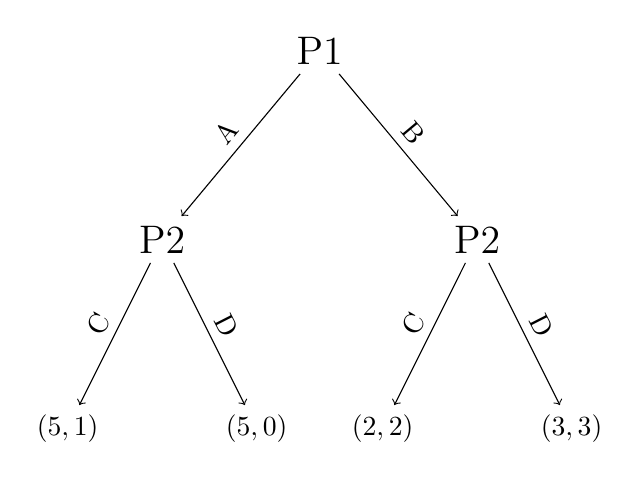
\begin{tikzpicture}[-, node distance = 2cm, scale=0.8]
    \node[anchor=north](P1){\Large{P1}};
    \node[anchor=north](P2_1) at (-2.5, -3) {\Large{P2}};
    \node[anchor=north](P2_2) at (2.5, -3) {\Large{P2}};

    \path[->] (P1) edge node [above, rotate=50] {A}(P2_1);
    \path[<-] (P2_2) edge node [above, rotate=310] {B}(P1);

    \node[anchor=north](F_1) at (-4, -6) {\((5,1)\)};
    \node[anchor=north](F_2) at (-1, -6) {\((5,0)\)};
    \node[anchor=north](F_3) at (1, -6) {\((2,2)\)};
    \node[anchor=north](F_4) at (4, -6) {\((3,3)\)};

    \path[->] (P2_1) edge node [above, rotate=60] {C}(F_1);
    \path[->] (P2_1) edge node [above, rotate=297] {D}(F_2);
    \path[->] (P2_2) edge node [above, rotate=60] {C}(F_3);
    \path[->] (P2_2) edge node [above, rotate=297] {D}(F_4);
\end{tikzpicture}
